\documentclass[a4paper]{article}
\usepackage[breaklinks=TRUE]{hyperref}
\usepackage{natbib}
\usepackage{rotating}
\usepackage[utf8]{inputenc} 
\usepackage{Sweave}
\begin{document}
\title{Tutorial to the RObsDat-package}
\author{Dominik Reusser}
%\VignetteIndexEntry{Tutorial to the RObsDat-package}
\maketitle
\section{Introduction}
Research data is a valuable asset. As \citet{Gold2007} put it:
\begin{quotation}
   ``[\ldots] data is the currency of science, even if publications are still the currency of tenure. To be able to exchange data, communicate it, mine it, reuse it, and review it is essential to scientific productivity, collaboration, and to discovery itself.''
\end{quotation}

This is also true for hydrological data. However, making data exchangeable and communication requires a well organized data management, for which funding is often not or only to a limited extend available. Efficient methods to manage hydrological data for small and medium scale projects has been missing up to now. What is required is a system that
\begin{itemize}
  \item stores data in a structured (adhering to standards) and efficient way
  \item allows centralized or decentralized data management
  \item is simple to set up with limited or intermediate database skills
  \item avoids date time errors due to wrong conversion
  \item provides flexible and efficient ways of data import and data export
  \item supports and documents data cleaning steps
  \item provides tools for data analysis
  \item runs independent of the operating system
  \item allows inspection of the code for debugging and further development
  \item provides documentation
\end{itemize}

The \href{http://cran.r-project.org/web/packages/RObsDat/index.html}{RObsDat} package is designed to fill this gap
in conjunction with the R environment and is currently in a
testing phase where code is made more efficient and more
stable. In order to use RObsDat, you need to understand the
format used for data storage. This will be presented in
section~\ref{sec:odm}. The role sharing between the R
environment and the package is briefly touched upon in
section~\ref{sec:sharing}. Different database
engines are supported by the package and basics
are presented in section~\ref{sec:db_engines}.
You might decide to initially skip
sections~\ref{sec:sharing} and
~\ref{sec:db_engines} and use the simple example
presented in section~\ref{sec:example} to learn
the practical usage of RObsDat. We conclude
(section~\ref{sec:conclusion}) with a
short outlook and an invitation to contribute.

\section{Observations Data Model}
\label{sec:odm}
Different database designs may be used to manage
hydrological (and other) data. RObsDat is designed
to store point observations which come with the
following properties. To store data with a
stronger spatial component (such as satellite
images and derivatives there off), a
(spatio-temporal) GIS system is recommended.

In general, hydrological observations come as a
triple including time, variables and space. This
triple is usually extended by information about
data quality and the data source/collection
method. CUASHI has presented a specification for
the Observations Data Model (ODM) which is
currently available as version 1.1
\citep{Tarboton2008}. 
This data model is
implemented by RObsDat, however the package has
been designed to be potentially compatible with other data
models. 
In addition, CUASHI recommends to use a
controlled vocabulary (CV) for the most important
attributes to enhance semantic consistency
and provides these through a web service. RObsDat
is able to import these CV.

Before you can store data with RObsDat, you need
to supply meta-data details for the location, the
variable, the quality and the source using the
commands \verb@addSite@, \verb@addVariable@,
\verb@addQualityControlLevel@, and \verb@addSource@. All
of these meta-data sets is stored in a separate
data table with additional links to specific
CV-tables. See the example in
section~\ref{sec:example} to get started.
The full data model is presented in
appendix~\ref{sec:odmmodel}.

\section{Role sharing between RObsDat, R and other packages}
A part of the power of managing your data with
RObsDat is the embedding environment R. It
provides great flexibility for data import,
scripting of standard processes, platform
independence. RObsDat relies on these advantages
of R and attempts to do the management of your
data in database well. When you receive data from
the database, use the power of R to do subsequent
(statistical) analyses and to create plots.
Important packages RObsDat depends on are related
to the management of time-objects and space-time
objects:
\label{sec:sharing}
\subsection{Date formats, zoo/xts}
When adding data values, RObsDat expects you to
provide time information in the \verb@POSIXct@
format. This is the interface between R and the
POSIX standard for date/time handling. You may
also store your data as time series data in form
of a \verb@zoo@ or \verb@xts@ object. See the
corresponding package documentations. You will need
a basic understanding of these to work with
RObsDat. Import from \verb@spacetime@ classes is
planned.

\subsection{spacetime}
The next version of the package will return data
as spacetime objects, which is a first step to
provide possibilities for efficient handling and
analysis of spatio-temporal data in R. See the
introductory journal article to the package for
more detail \citep{Pebesma2012}.

\section{Database engines}
\label{sec:db_engines}
RObsDat has been tested and made compatible with
three different, open source database engines:
SQLite, MySQL and PostgreSQL. The most simple
set-up is by using SQLite, which stores all the
information in a single file with the extension
db. The default is a file in the current working
directory and the name \verb@RODM.db@. You can
share the db-file, such that other users can also
access your database. Free graphical user
interfaces to SQLite databases exist for most
operating systems and can be found on the web.

In case you don't know what to do,
\verb@getDefaultDB()@ will install a preconfigured
database file shipped with the package. This
command also work if your db file is called \verb@RODM.db@ and
is situated in your working directory.
\begin{Schunk}
\begin{Sinput}
> getDefaultDB()
\end{Sinput}
\end{Schunk}

To connect to a different SQLite
database, you may use the following set of
commands:
\begin{Schunk}
\begin{Sinput}
> require("RObsDat")
> require("RSQLite")
> m <- dbDriver("SQLite")
> dbname = "database.db"
> con <- dbConnect(m, dbname = dbname)
> sqhandler <-  new("odm1_1Ver", con=con)
> options(odm.handler=sqhandler)
\end{Sinput}
\end{Schunk}


However, concurrent data
management by multiple users is not advisable with
such a set-up. Running a database server is
recommended in such a case. Contact your system
administrator if you need to set-up a database
server. To connect to a running server, you may
use the following commands.
\begin{Schunk}
\begin{Sinput}
> #connect to postgreSQL database
> require("RObsDat")
> require("RPostgreSQL")
> m <- dbDriver("PostgreSQL")
> con <- dbConnect(m, user="a_user", password="secret", dbname="obsdat")
> sqhandler <-  new("odm1_1Ver", con=con)
> options(odm.handler=sqhandler)
> #connect to MySQL database
> require("RObsDat")
> require("RMySQL")
> m <- dbDriver("MySQL")
> con <- dbConnect(m, user="a_user", password="secret", dbname="obsdat")
> sqhandler <-  new("odm1_1Ver", con=con)
> options(odm.handler=sqhandler)
\end{Sinput}
\end{Schunk}

\section{An example session}
\label{sec:example}
We start by obtaining a preconfigured database,
shiped with the package as \verb@RODM.db@ into our
current working directory. All modification will
be stored in this file. If you again use
\verb@getDefaultDB()@ in the same
working directory, a connection will be made to
the existing database file and you will have
access to all the former modifications. If you
want to start with a blank database, make sure to
delete the file. However, RObsDat is designed to
be smart about repeated execution of commands and
will avoid duplication of records. Let's get
started:
\begin{Schunk}
\begin{Sinput}
> getDefaultDB()
\end{Sinput}
\end{Schunk}

Before adding data values, we need to set up the
meta-data. We will check what the correct names of
the meta-data are:

\begin{Schunk}
\begin{Sinput}
> #Store metadata in database
> getMetadata("SpatialReference", SRSName="WGS84", exact=TRUE)
\end{Sinput}
\begin{Soutput}
  ID SRSID SRSName IsGeographic Notes
1  3  4326   WGS84         TRUE      
\end{Soutput}
\begin{Sinput}
> addSite(Code="testLocation", Name="Virtual test site", x=-5, y=46,
+ 	LatLongDatum="WGS84", Elevation=1500, State="Germany")
> getMetadata("Units", Abbreviation="cm")
\end{Sinput}
\begin{Soutput}
    ID                                                    Name
1    9                                               arcminute
2   14                                       square centimeter
3   32                             watts per square centimeter
4   47                                           centimeter   
5   86                                   centimeter of mercury
6   87                                     centimeter of water
7  109                                    centimeters per hour
8  110                                  centimeters per second
9  136                  calories per square centimeter per day
10 137               calories per square centimeter per minute
11 138               milliliters per square centimeter per day
12 149                               absorbance per centimeter
13 187                             microsiemens per centimeter
14 190                              cubic centimeters per gram
15 193                              grams per cubic centimeter
16 226 the ratio between UV absorbance at 254 nm and DOC level
17 253       absorbance per centimeter per mg/L of given acid 
18 263                             millisiemens per centimeter
19 281                            cubic centimeters per second
20 292                              decisiemens per centimeter
21 294                            Joules per square centimeter
22 318                              hits per square centimeter
23 319                     hits per square centimeter per hour
                      Type  Abbreviation
1                    Angle        arcmin
2                     Area          cm^2
3              Energy Flux        W/cm^2
4                   Length            cm
5          Pressure/Stress         cm Hg
6          Pressure/Stress        cm H2O
7                 Velocity         cm/hr
8                 Velocity          cm/s
9              Energy Flux    cal/cm^2 d
10             Energy Flux  cal/cm^2 min
11          Hyporheic flux     ml/cm^2 d
12   Extinction/Absorbance          A/cm
13 Electrical Conductivity         uS/cm
14         Specific Volume        cm^3/g
15           Concentration        g/cm^3
16  Specific UV Absorbance L/(mg DOC/cm)
17              Absorbance   100/cm mg/L
18 Electrical Conductivity         mS/cm
19                    Flow      cm^3/sec
20 Electrical Conductivity         dS/cm
21         Energy per Area        J/cm^2
22           Precipitation     hits/cm^2
23                Velocity  hits/cm^2 hr
\end{Soutput}
\begin{Sinput}
> getMetadata("VariableName", Term="Distance")
\end{Sinput}
\begin{Soutput}
      Term
1 Distance
                                                                                               Definition
1 Distance measured from a sensor to a target object such as the surface of a water body or snow surface.
\end{Soutput}
\begin{Sinput}
> addVariable(Name="Distance", Unit="cm", ValueType="Field Observation",
+ 	GeneralCategory="Instrumentation", Code="test_dist")
> addQualityControlLevel(ID=6,Code="ok", Definition="The default")
> addISOMetadata(TopicCategory="Unknown", Title="Testdata",
+ 	Abstract="This data is created to test the functions of RObsDat")
> addSource(Organization="Your Org", SourceDescription="Madeup data", 
+ 	SourceLink="RObsDat Documentation", ContactName="Yourself",
+ 	Metadata="Testdata")
\end{Sinput}
\end{Schunk}

With this set of commands, we are done preparing
meta-data for a first Variable and Location. Note
that the information about the source is stored in
two tables, one including the 
\href{http://en.wikipedia.org/wiki/Dublin_Core}{Dublin Core}
information and the other remaining meta-data.
From the example, it should be simple to add
meta-data for other locations or other variables.
For the tutorial, we are content with one site and
one variable.

As a next step, we can start to add data. Let's
create a tutorial data set and store it a xts.
We introduce two data errors that we want to
correct in a subsequent test. 

\begin{Schunk}
\begin{Sinput}
> library(xts)
> example.data <- xts(1:366, seq(as.POSIXct("2010-01-01", tz="UTC"), 
+ 		as.POSIXct("2011-01-01", tz="UTC"), length.out=366))
> example.data[50] <- 100
> example.data[200] <- 40
\end{Sinput}
\end{Schunk}

With loggers, we often obtain multiple files with
partially redundant data (the later dataset
containing some of the information from a previous
dataset). RObsDat is able to detect redundant
data. As long as no conflicts arise, the package
is silent about redundant entries. If present, existing
conflicts are presented and the user is asked
about the desired action. We simulate this by
first importing the first 100 data sets, modifying
our data and then importing the remaining data
set.

\begin{Schunk}
\begin{Sinput}
> addDataValues(example.data[1:100], Site="testLocation", Variable="test_dist",  
+ 	Source="Madeup", QualityControlLevel="ok")
\end{Sinput}
\begin{Soutput}
Importing column  1 out of 1 
\end{Soutput}
\begin{Sinput}
> #Avoid duplicates autmatically
> example.data[75] <- 100
> addDataValues(example.data, Site="testLocation", Variable="test_dist",  
+ 	Source="Madeup", QualityControlLevel="ok")
\end{Sinput}
\begin{Soutput}
Importing column  1 out of 1 
Data to import is not matching data in database for 1 values (See plot)
What shall I do?
  1) Dischard data to import and import remaining, missing data
  2) Overwrite values in database with new values
  0) Stop and let you modify the data to import before another attempt
Enter a number (0-2) for your choise.
\end{Soutput}
\end{Schunk}

Note the ''split
responsibility'' between the R environment and
RObsDat (section~\ref{sec:sharing}). 
You will use the power and flexibility of
R to get the data into the environment and convert
dates into a POSIX-format, while the package
provides support mechanisms to get the data in a
consistent form into the database.
Note that the import method is quite smart about
data configurations and automatically detects
whether meta-data is valid for columns or rows or
is provided as full table (check this out yourself
and report unexpected behaviour to the maintainer).
Also, typos and multiple versions for site and
variable names are interactively caught and the
database remembers synonyms for data sets.
Data in the database can be accessed and filtered
in an intuitive way:

\begin{Schunk}
\begin{Sinput}
> inDB <- getDataValues(Site="test")
> plot(inDB)
\end{Sinput}
\end{Schunk}

Raw data often needs to be cleaned before it can
be used. RObsDat supports this and allows to
reconstruct data modification operations. The
following lines demonstrate this:

\begin{Schunk}
\begin{Sinput}
> #Version management
> to.correct <- which(inDB@values < 100 & 
+ 	index(inDB@values) > as.POSIXct("2010-06-01"))
> inDB@values[to.correct] <- 200
> inDB@values[50] <- 50
> updateDataValues(inDB, "Correction of wrong value")
> ver2 <- inDB
> ver2@values[50:60] <- 90
> updateDataValues(ver2, "Changing more data")
> ver3 <- inDB
> ver3@values[50:60] <- 190
> updateDataValues(ver3, "Ups, I used 90 instead of 190 by mistake")
> deleteDataValues(inDB[250],  "And finally remove a value")
\end{Sinput}
\begin{Soutput}
NULL
\end{Soutput}
\begin{Sinput}
> getDataVersions()
\end{Sinput}
\begin{Soutput}
  VersionID          ValidUntil                           VersionComment
1         1 2013-10-23 09:35:34                          Initial Version
2         2 2013-10-23 09:35:34                Correction of wrong value
3         3 2013-10-23 09:35:35                       Changing more data
4         4 2013-10-23 09:35:36 Ups, I used 90 instead of 190 by mistake
5         5                <NA>               And finally remove a value
\end{Soutput}
\begin{Sinput}
> versionQuery <- getDataValues(Site=1, VersionID=1)
> plot(versionQuery)
> versionQuery <- getDataValues(Site=1, VersionID=2)
> plot(versionQuery)
\end{Sinput}
\end{Schunk}

\section{Conclusion}
\label{sec:conclusion}
Ideally RObsDat will be a valuable tool for you to
manage your data. It is currently still under
development. You can contribute by testing the
package and reporting what works and what doesn't,
by improving the documentation, by making some
funding available for further development...

\appendix
\section{The full data model}
\label{sec:odmmodel}
\begin{sidewaysfigure}
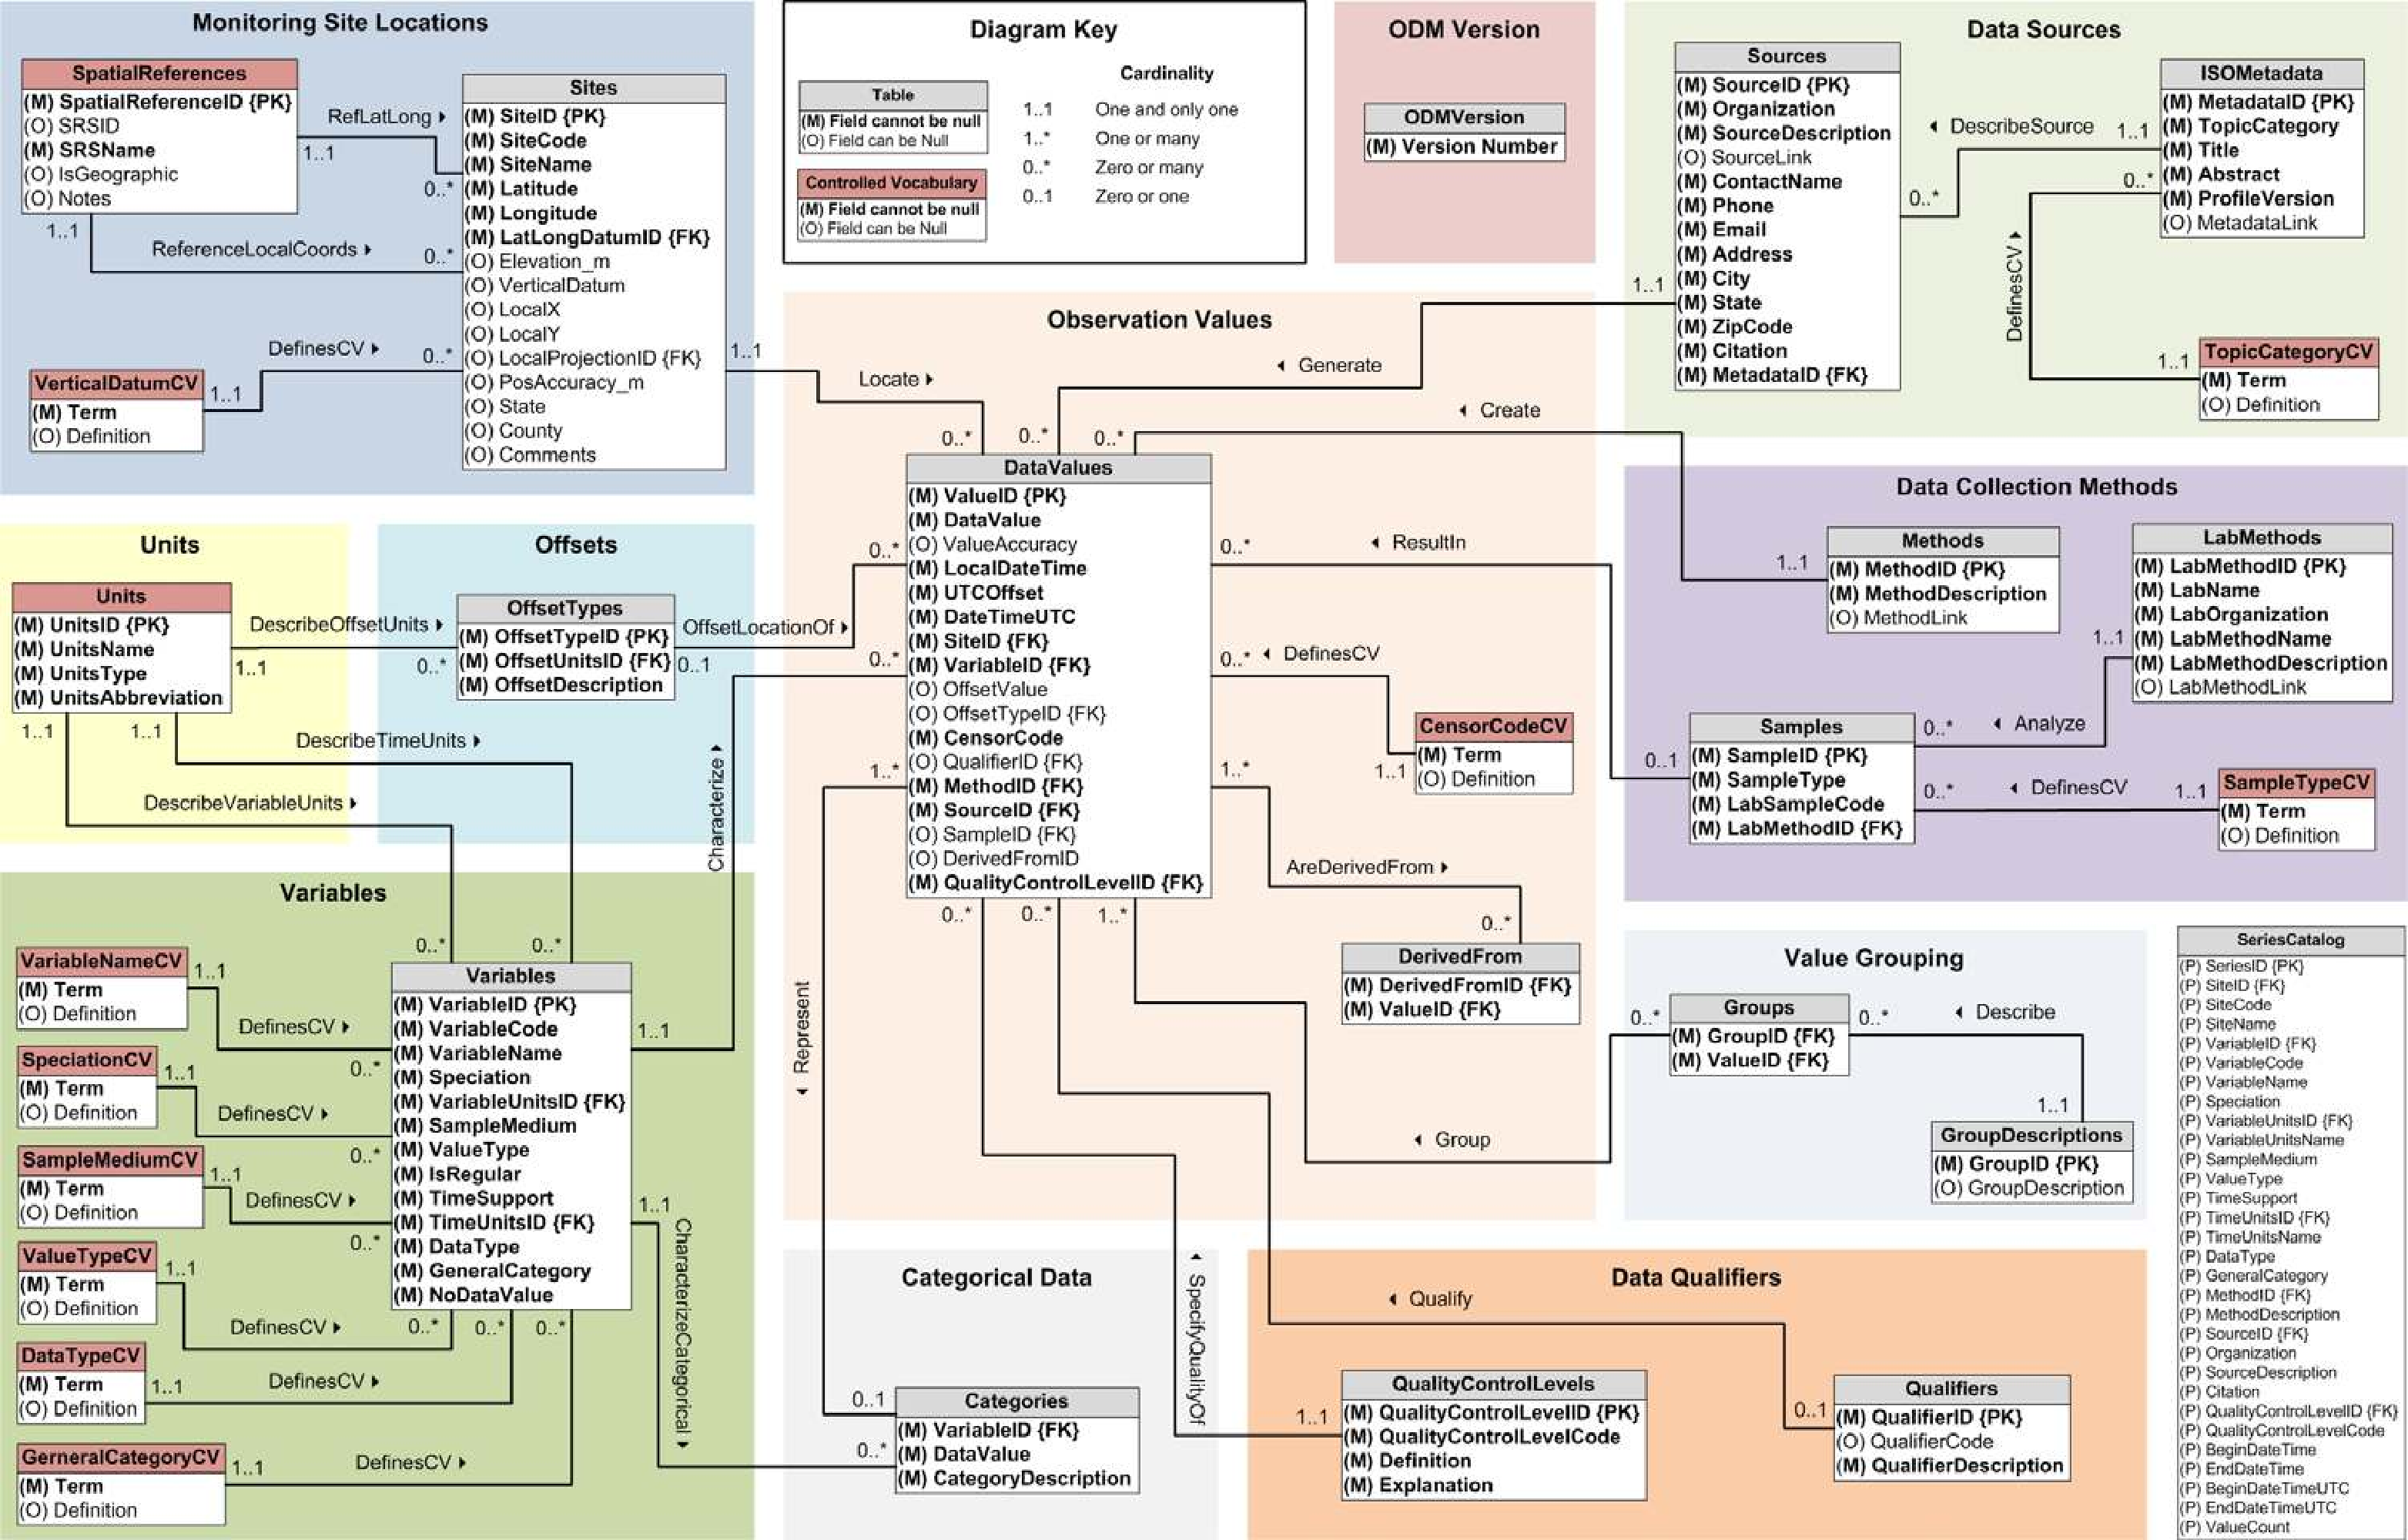
\includegraphics{odm}
\caption{Observations Data Model as specified in \citet{Tarboton2008}. Image source: \citet{Tarboton2008}}
\end{sidewaysfigure}

\bibliographystyle{plainnat}
\bibliography{RObsDat}
\end{document}
